\documentclass{beamer}
\usetheme{Madrid}
\usepackage{graphicx}
\usepackage[T1]{fontenc}
\usepackage[polish]{babel}
\usepackage[polish]{datetime2}


\title{Marketing investment model (MIM)}
\author{Famiglia Zippone}
\institute{UWr}
\date{\today}

\begin{document}

\begin{frame}
\titlepage
\end{frame}


\begin{frame}{Główna idea}

{\center\it\bf
Wyobraź sobie że jesteś przedstawicielem firmy Coca-Cola...
}
\vspace{0.5cm}

\pause

\begin{itemize}
    \item Czy wydasz 50 000 zł na reklamę w Warszawie?
    \item Czy lepiej wydać 10 000 zł na reklamę w Radomiu?
\end{itemize}
\vspace{0.5cm}

\pause

{\color{red} Pomysł:} Narzędzie, które oszacuje zwrot z inwestycji w danej lokacji.  

\end{frame}


\begin{frame}{Jak to działa?}
\begin{figure}
    \centering
    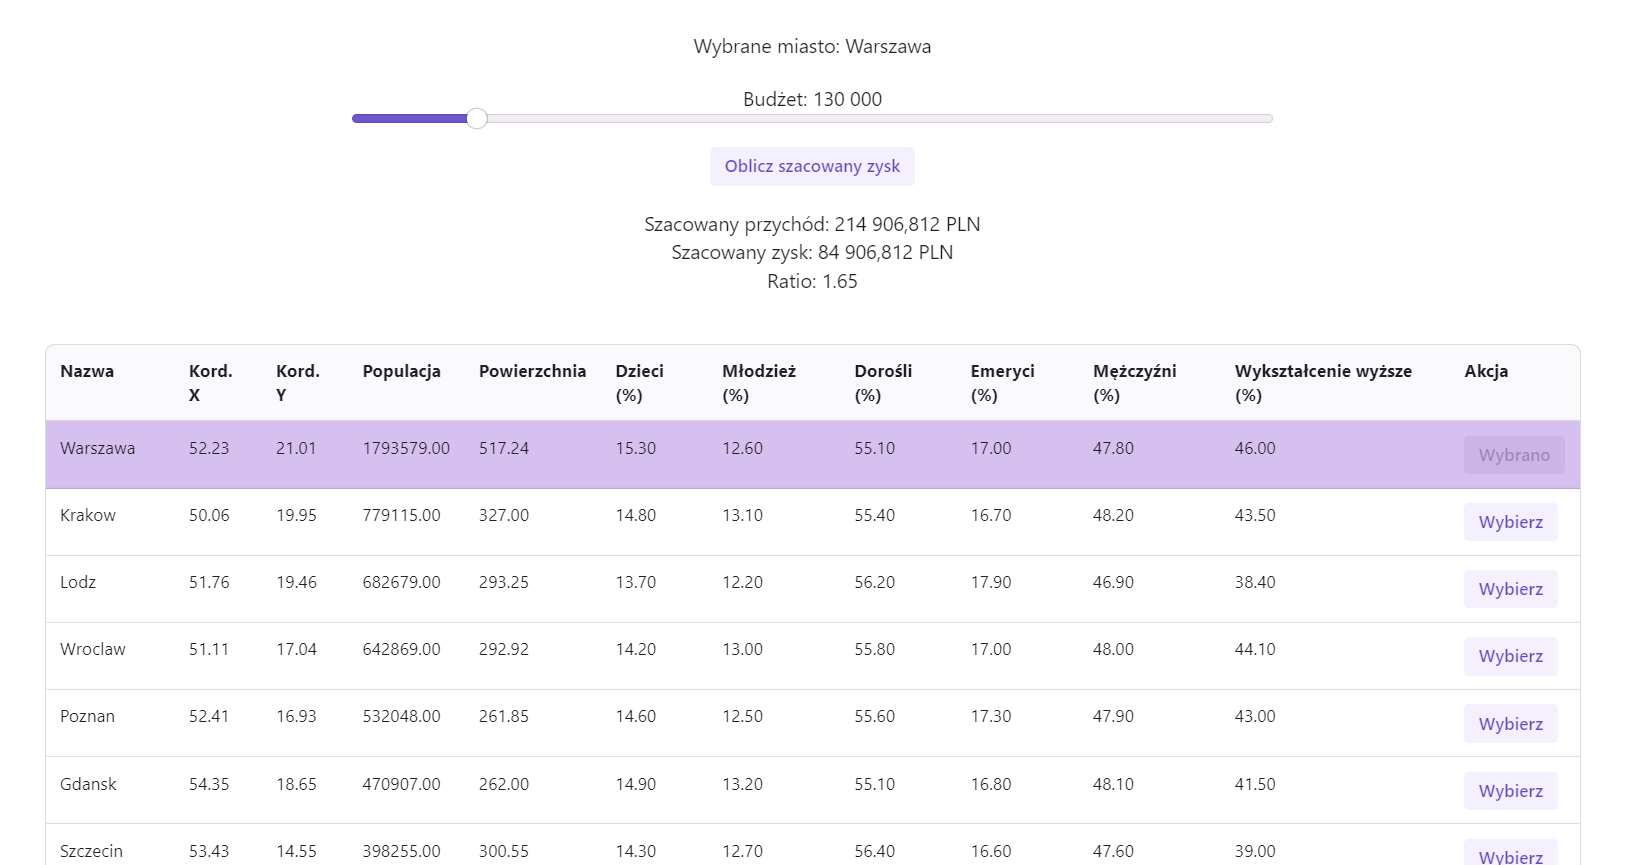
\includegraphics[width=\linewidth]{site_demo.png}
\end{figure}
\end{frame}



\begin{frame}[t]{Jak wygląda nasz model?}

{\Large Model oparty jest na sekwencyjnej sieci neuronowej.

\vspace{0.5cm}

Specyfikacja:}

\vspace{1cm}
\begin{itemize}
    \setlength\itemsep{1em}
    \item Biblioteka Keras do obliczeń
    \item Biblioteka Pandas do manipulacji danych
    \item Parametrami charakterystyka miasta
\end{itemize}
\end{frame}

\begin{frame}{Średni błąd kwadratowy}
\begin{figure}
    \centering
    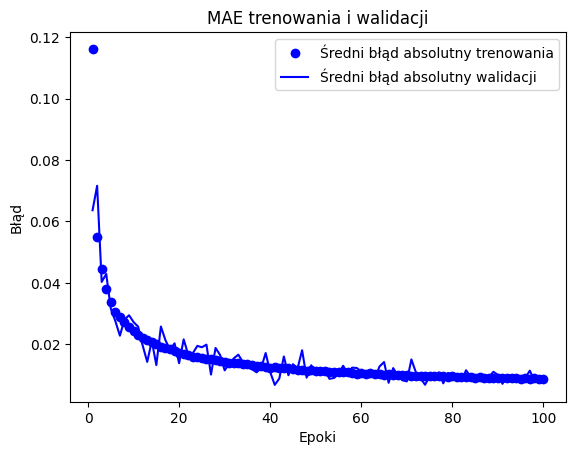
\includegraphics[width=0.7\linewidth]{mae.png}
\end{figure}
\end{frame}


\begin{frame}[t]{Jak to działa?}

{\Large Zalety:}
\vspace{0.5cm}
\begin{itemize}
    \item Personalizacja - danymi są poprzednie kampanie reklamowe
    \item Elastyczność - producent sam dobiera wartość oraz miejsce inwestycji
    \item Uniwersalność - narzędzie działa dla dowolnego produktu
\end{itemize}

\pause

\vspace{1cm}

{\Large Wady:}
\vspace{0.5cm}
\begin{itemize}
    \item Mało rozbudowane (jeszcze ;))) )
    \item Wymaga danych nt. historii inwestycji
\end{itemize}

\end{frame}

\begin{frame}{Co dalej?}
Uważamy, że jest to prototyp pomysłu, który można rozwijać w wielu kierunkach. Przykładowo:
\begin{itemize}
    \item Doskonalenie danych dotyczących profilu psychologicznego mieszkańców
    \item Integracja z dane.gov
    \item Wyszczególnienie typu strategii marketingowej (bilbordy, filmy, plakaty, etc.)
\end{itemize}

\end{frame}


\begin{frame}{Wykres satysfakcji od czasu}
\begin{figure}
    \centering
    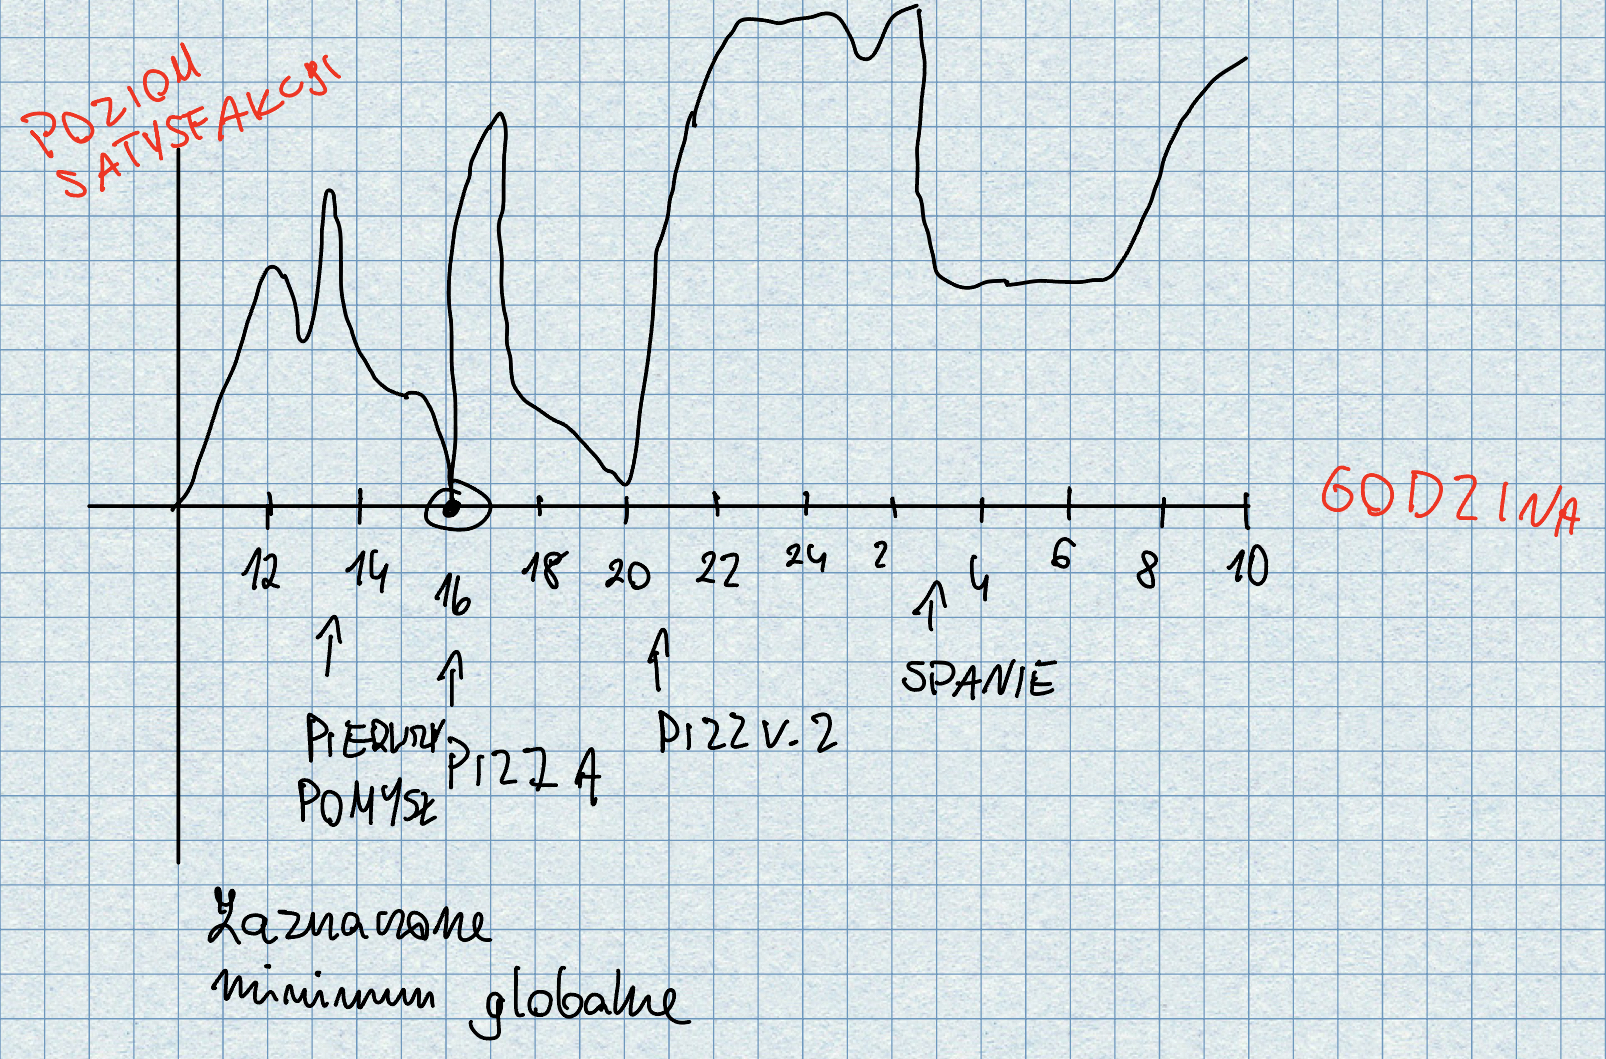
\includegraphics[width=0.7\linewidth]{satisfaction.jpeg}
\end{figure}
\end{frame}


\end{document}